\chapter{Tests}
\label{chap:tests}
For this work, the Context Broker was implemented. A Broker management interface was created, it is shown in Figure \ref{fig:broker}. For testing this implementation, both a Provider and a Consumer interfaces were created, respectively illustrated on Figure \ref{fig:provider} and Figure \ref{fig:consumer}.

The Broker management interface allows a system manager to see the Providers registered in the Broker, shown in Figure \ref{fig:providers}, as well as the context information they have updated to it (Figure \ref{fig:registries}). The manager also has access to the Subscriptions made by Consumers and the \textbf{log} of the Broker system, both shown on Figure \ref{fig:subscriptions} and Figure \ref{fig:log}. \par

\begin{figure}[H]
	\centering
	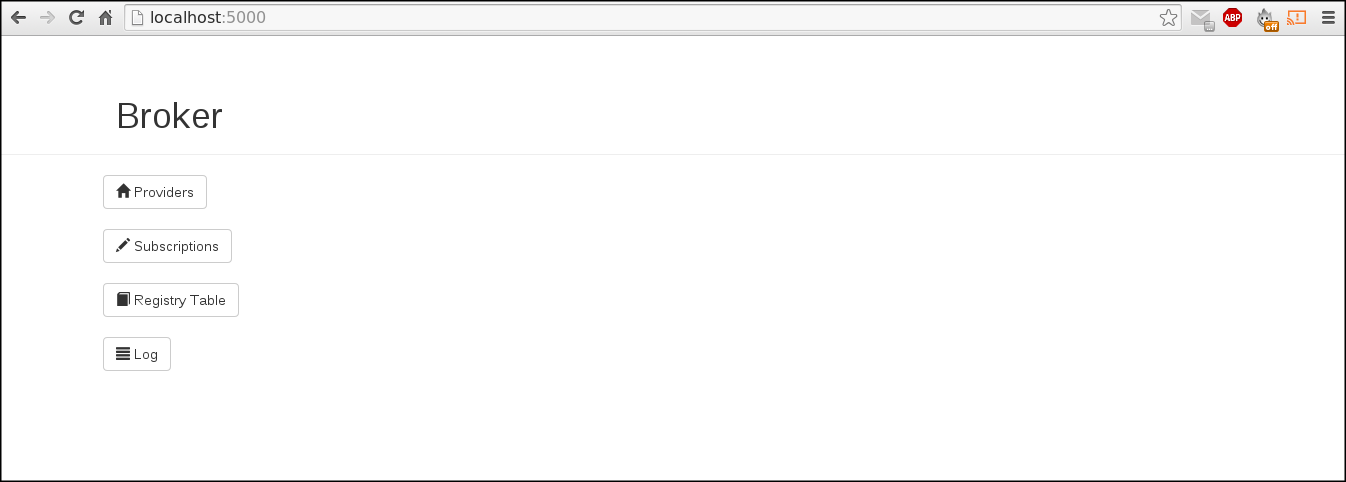
\includegraphics[scale=0.2]{broker.png}
	\caption{Broker Interface}
	\label{fig:broker}
	
\end{figure}

\begin{figure}[H]
	\centering
	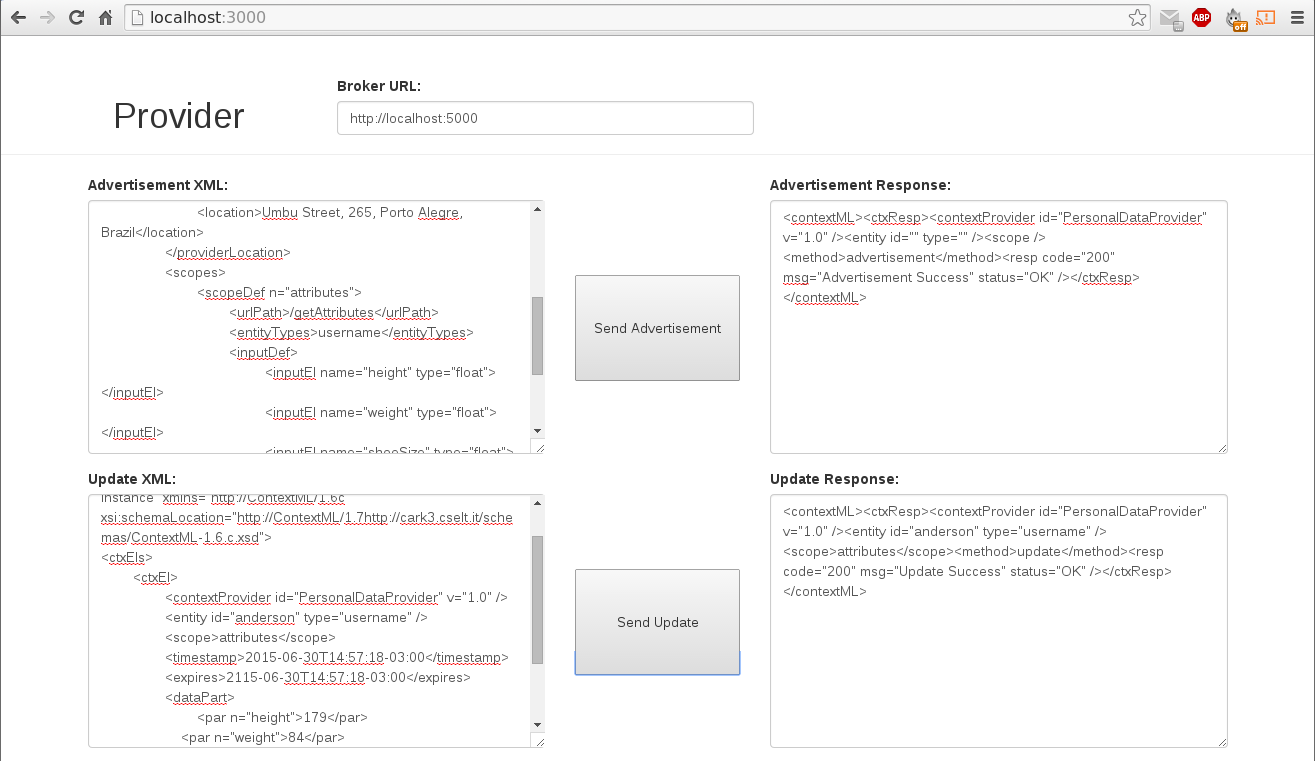
\includegraphics[scale=0.2]{provider.png}
	\caption{Provider Interface}
	\label{fig:provider}
	
\end{figure}

\begin{figure}[H]
	\centering
	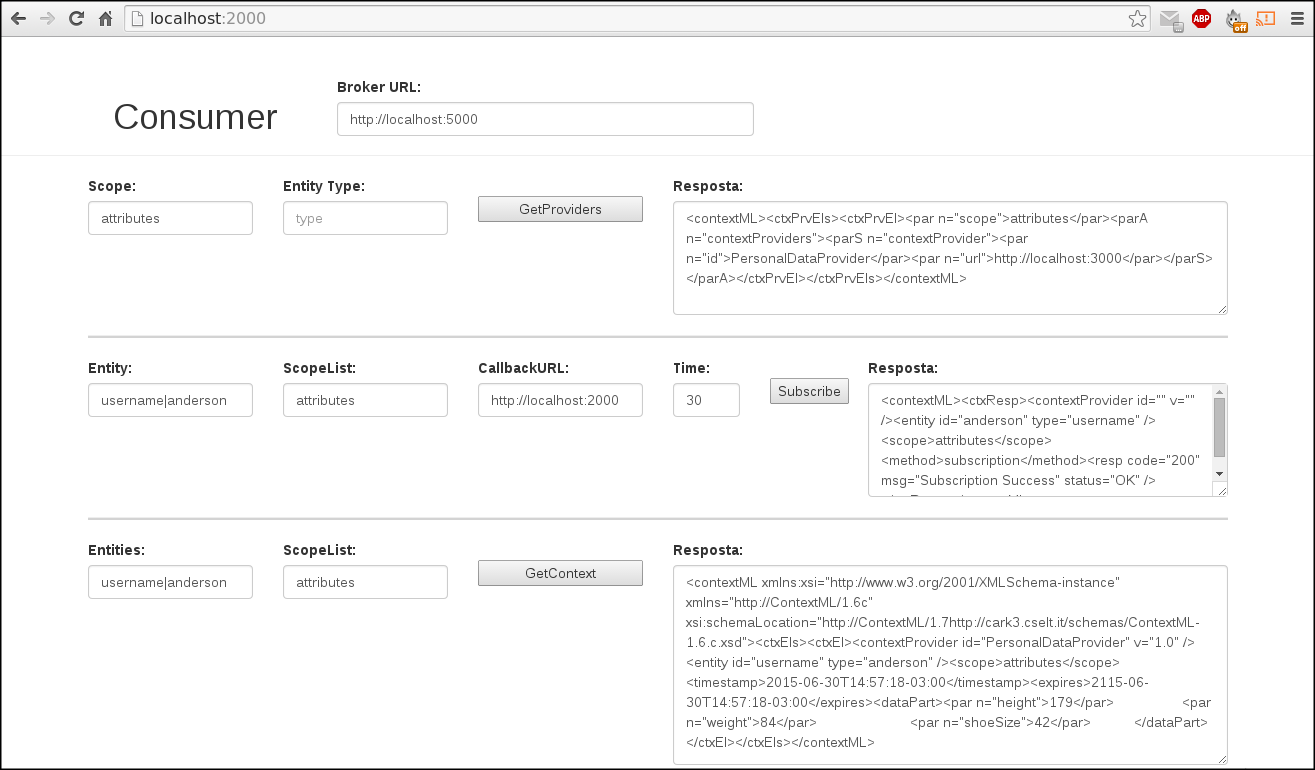
\includegraphics[scale=0.2]{consumer.png}
	\caption{Consumer Interface}
	\label{fig:consumer}
	
\end{figure}

\begin{figure}[H]
	\centering
	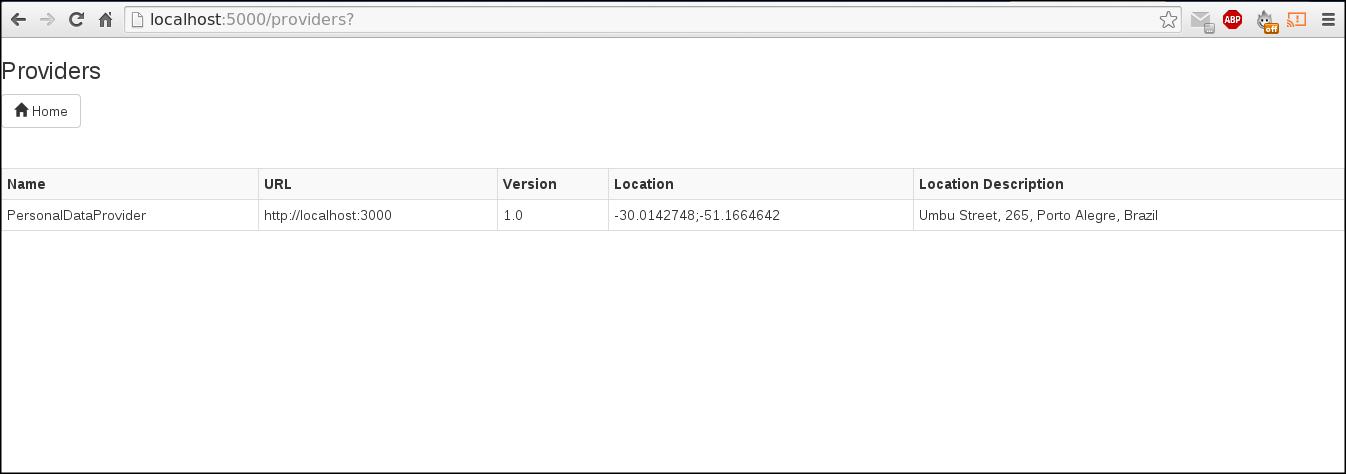
\includegraphics[scale=0.2]{brokerprovs.png}
	\caption{Providers Table}
	\label{fig:brokerprovs}
	
\end{figure}

\begin{figure}[H]
	\centering
	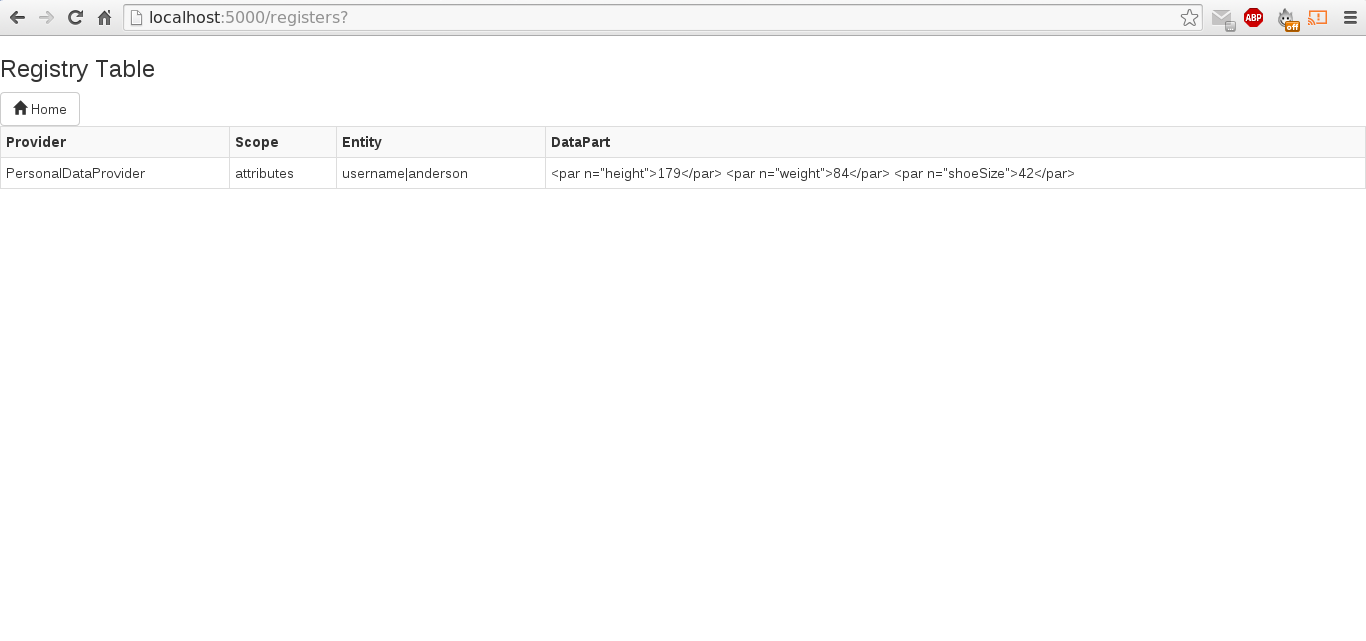
\includegraphics[scale=0.2]{registries.png}
	\caption{Registry Table - Context Information}
	\label{fig:registries}
	
\end{figure}

\begin{figure}[H]
	\centering
	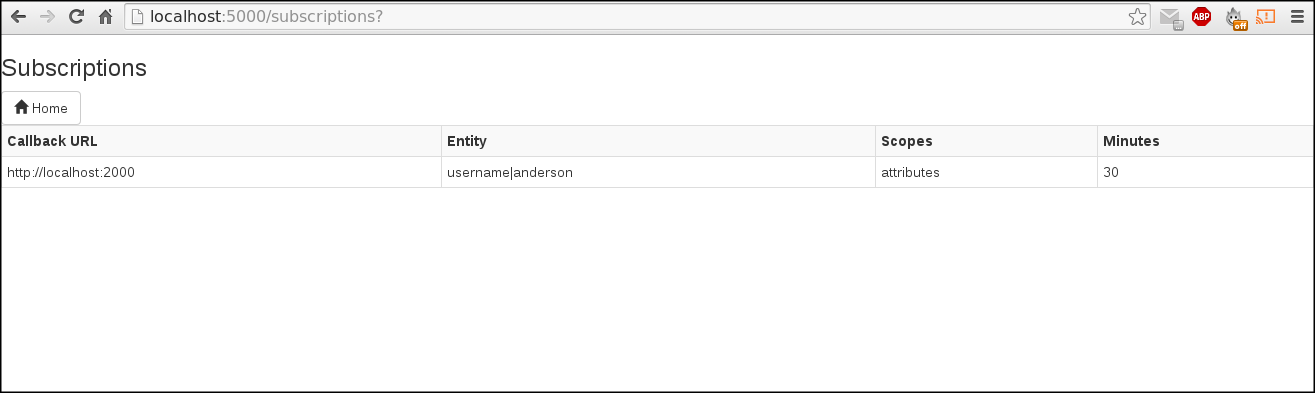
\includegraphics[scale=0.2]{subscriptions.png}
	\caption{Subscriptions Table}
	\label{fig:subscriptions}
	
\end{figure}

\begin{figure}[H]
	\centering
	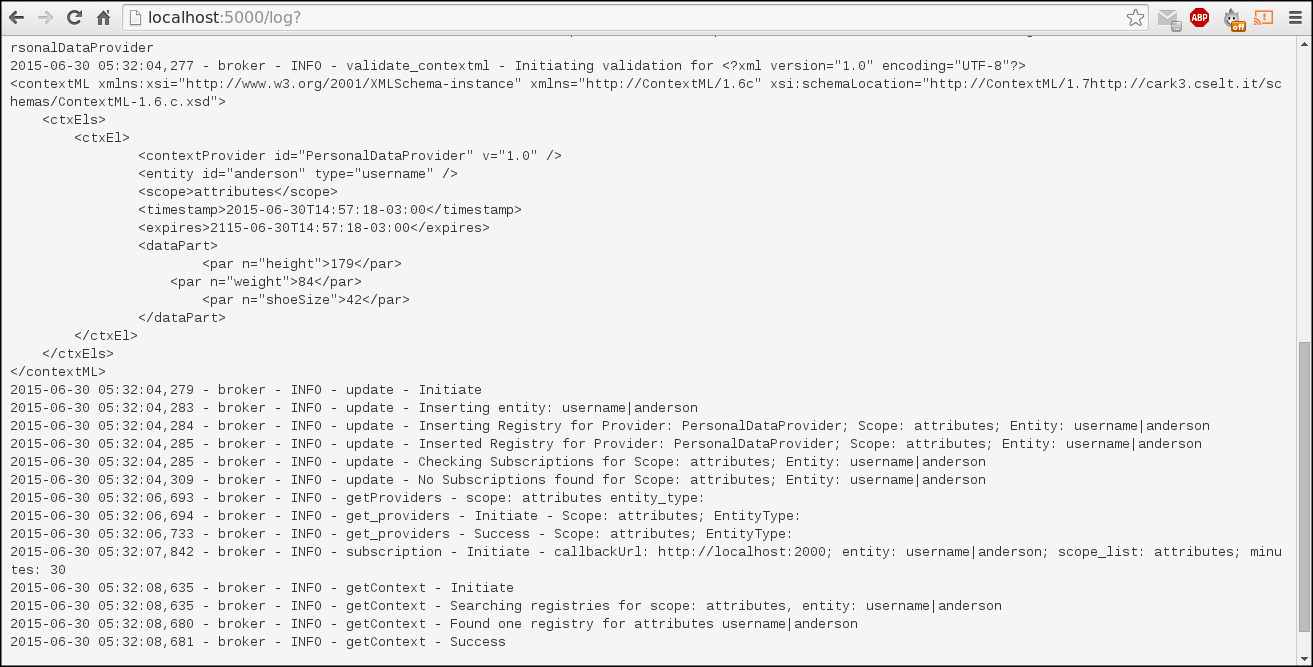
\includegraphics[scale=0.2]{log.png}
	\caption{Broker Log}
	\label{fig:log}
	
\end{figure}

 